\section{Energy efficiency}
As in exercise 1, when discussing energy efficiency, we will be focusing on amperage, since it's more relateable to, among other things, battery capacity.

\subsection{Readings}

In the final iteration of our implementation, we were able to have the microcontroller enter energy mode 4 with no extra peripherals enabled, allowing it to idle at about $2\mu A$. Figure \ref{idle-fig} shows a log-scale plot of the amperage while idle and figure \ref{playing-fig} shows the active amperage.

\begin{figure}[h!]
    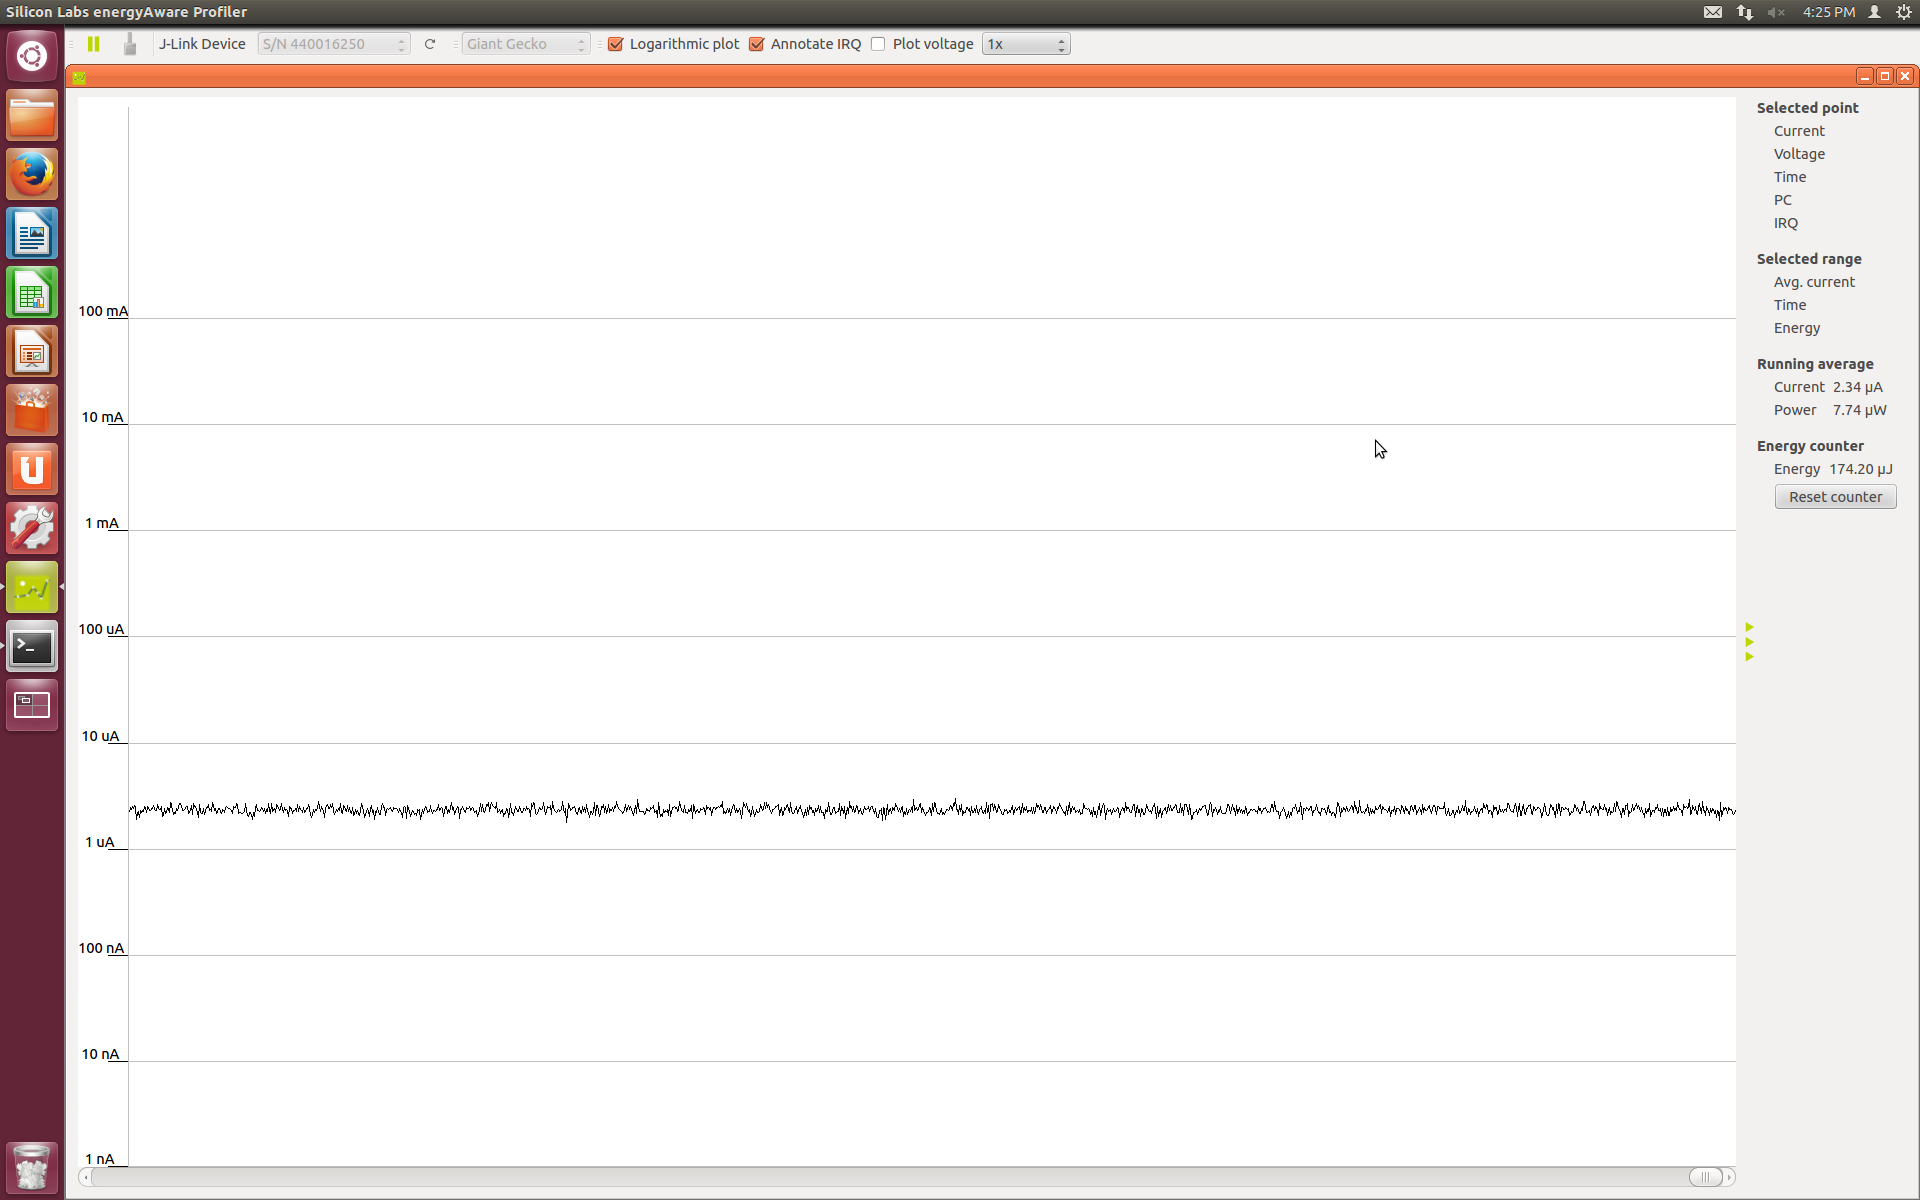
\includegraphics[width=\linewidth]{img/idle.png}
    \caption{Idle amperage plotted by the eAProfiler tool.}
    \label{idle-fig}
\end{figure}

\begin{figure}[h!]
    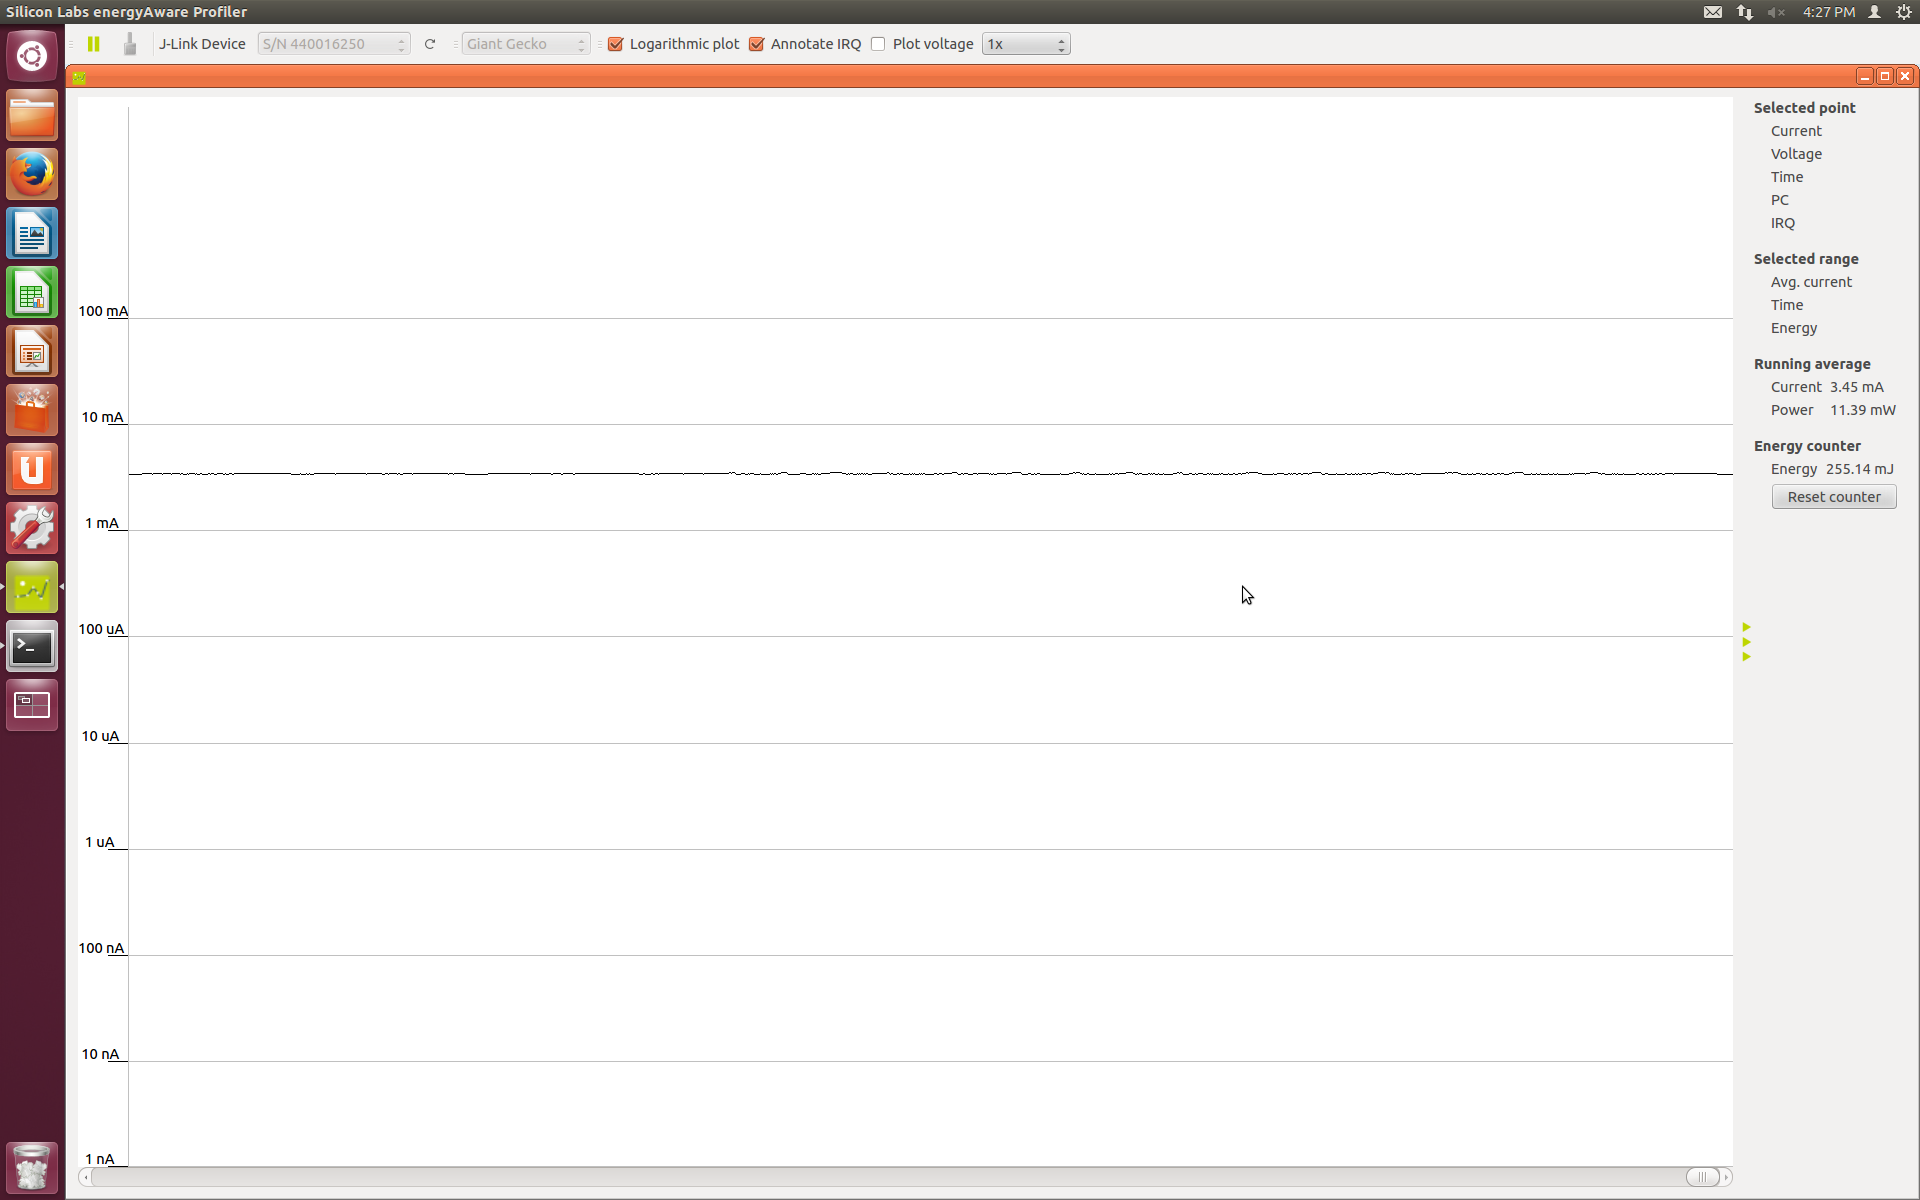
\includegraphics[width=\linewidth]{img/playing.png}
    \caption{Active amperage plotted by the eAProfiler tool.}
    \label{playing-fig}
\end{figure}

\subsection{Expected lifetime on a CR2032 battery}

In our report for exercise 1, we used the CR2032 battery as an example in the energy efficiency section. \cite[p.~13]{exercise1report} Since our idle power consumption is at the same level in this exercise as in the previous, our conclusion from that report still stands; in idle mode, the battery will deteriorate before discharging from the microcontrollers usage. This time however, the functionality of our program is rather different, and it spends a larger amount of time not idling. As can be seen from figure \ref{playing-fig}, the amperage while playing is around $3.5mA$. Using the same reference battery capacity \cite{cr2032} as in exercise 1, and the playing amperage, formula \ref{playing-formula} gives us an expected lifetime with continuous playing, of about 2 days, 20 hours.

\begin{gather}
\label{playing-formula}
\frac{240mAh}{3.5mA} = 68.6 hours
\end{gather}

\subsection{Discussion}

The final iteration of our program implements a simple way of playing both short sound effects and longer musical pieces, with low power consumption while idle to boot. We learned a lot about general sound theory, DAC usage, microcontroller programming in C and about many of the relevant peripherals on the EFM32GG. Our implementation lacked in a few places however, namely energy efficiency while playing and variation of sound.

\subsubsection{Active energy consumption}

As described in section \ref{playing-the-sounds}, we chose to disable deepsleep while each song plays. The result of this is an average amperage of $3.5mA$ while playing sounds, which is rather high. This could have been improved in several ways, given more time.

One possible way to improve active power consumption would have been to use a dfferent timer. The regular timer works along these lines; the timer incrementes its counter value once every clock cycle until it reaches the value set in the TOP register. Since the timer relies on the clock cycles from the High Frequency Peripheral Clock, this timer must be run in energy mode 0. We spent some time investigating other possibilities, amongst them using the low energy timer wich can be used while in energy mode 1 or 2, seeing as it uses one of the low frequency clocks as a source. These clocks run at $32.768 kHz$ or lower, so opting to use the low energy timer would mean sacrificing sound resolution for energy efficiency.

In the compendium the possibility of using Direct Memory Access (DMA) was mentioned as a possible method to reduce power consumption. We looked into this, but did not implement it, as our program relies on the CPU to change the current playing note. If the program had instead played songs as long continuous sample sequences, DMA would be useful as the CPU could have longer periods of time idling.

Finally, we could also have disable any unused ram, using the memory system controller (MSC). We investigated how to do this towards the end of the development process, but opted for putting in more hours working on this report instead.

\subsubsection{Sound features}

Our implementation has several convenient features, among them a very simple system for adding new songs and controlling how long a song lasts. However, as our system only implements sine waves, most music implemented, while being tonally perfect, will have little room for variation. Given more time, we could have implemented a more sophisticated system for representing songs, involving additional wavetypes (i.e. square and sawtooth) and tweakable parameters.
